\chapter{Test dei metodi di spam detection}
\lstset{basicstyle=\small\ttfamily,keywordstyle=\color{black}\bfseries,commentstyle=\color{darkgray},stringstyle=\color{black},showstringspaces=true} 
Nei capitoli precendenti sono stati illustrati vari metodi che di spam detection classificati basandosi sui segnali in ingresso che essi hanno bisogno per poter identificare le pagine web; quindi si hanno tre classi: metodi basati sul contenuto, metodi basati sul grafo e metodi che utilizzano segnali diversi dai primi due. Tra questi metodi ne sono stati presi in esame due: \textit{Trustrank} e \textit{Anti-trust rank}. 

Si è scelto, quindi, di valutare l'efficacia di due  algoritmi \textit{linked base} (\textit{Trustrank} e \textit{Anti-trust rank}) se essi operassero in modo online. Più precisamente i vari test consistono nel verificare quanto questi due algoritmi di tipo offline riescano ad approssimare il loro comportamento se li facessimo operare in modo online ovvero durante la fase di crawling. Le domande che ci poniamo eseguendo questi test su i due algoritmi di spam dection offline (\textit{Trustrank} e \textit{Anti-trus rank}) sono:
\begin{itemize}
 \item possono questi algoritmi essere in grado di operare in modalità online?
 \item durante l'esecuzione in modalità online, quanto riescono ad approssimare il loro comportamento offline?
 \item è conveniente utilizzare questi algoritmi in modalità online?
\end{itemize}

E' doveroso specificare che un algoritmo di spam detection lavora offline se questo viene eseguito dopo l'attività di crawling (e quindi dopo che si ha a disposizione l'intero grafo ottenuto dai collegamenti tra le pagine), mentre un algoritmo di spam detection lavora online se questo viene eseguito durante il processo di crawling e quindi riesce a determinare all'istante se una pagina deve essere considerata spam o non spam. Dal momento che si è scelto di esaminare degli algoritmi \textit{linked base}, e sapendo che questi formulano delle conclusioni sulla natura delle pagine (ovvero se sono spam o non spam) esaminando la struttura dell'intero grafo, è interessante notare come questi si comportino se il grafo su cui fare le valutazioni è incompleto.
%altre considerazioni

Il capitolo è diviso nel seguente modo: nella prima parte verrà illustrato come è stato scelto di simulare il crawler per poter eseguire gli algoritmi offline duratne la fase di crawling; nella seconda parte verrà spiegato come sono stati implementati i test; infine verrano illustrati tutti i test.

\section{Simulazione del crawler}
Per simulare il comportamento di crawler, e quindi eseguire gli algoritmi di \textit{Trustrank} e \textit{Anti-trust rank}, abbiamo implementato una semplice visita sul grafo in ampiezza ovvero una BFS \cite{bfsCormen} (Breadth-First Search). La visita in ampiezza dato un grafo \(G=(V,E)\), dove \(V\) è l'insieme dei vertici del grafo ed \(E\) l'insieme degli archi del grafo, e un vertice \(s\) da cui far partire la visita, scopre tutti i vertici che sono raggiungibili da \(s\). La visita in ampiezza scopre tutti i vertici che si trovano a distanza \(f\) dal vertice di partenza e successivamente scopre i vertici che si trovano a una distanza successiva \(f+1\). In sostanza dato il nodo di partenza \(s\), la visita in ampiezza, scopre tutti i nodi vicini al nodo \(s\) e successivamente per ogni nodo vicino scoperto trova i vicini che non sono ancora stati visitati; questo processo viene iterato finche tutti i nodi del grafo raggiungibili da \(s\) sono visitati. \\
Quindi anziche implementarci l'algoritmo BFS abbiamo utilizzato l'implementazione definita nel framework WebGraph. In particolare è stata utilizzata la classe ``ParallelBreadthFirstVisit'' che esegue una visita in ampiezza utilizzando il parallelismo derivato dai processori multicore.

\section{I test}
Come gia introdotto lo scopo dei test consiste che dato un algoritmo di spam detection che opera in modo offline valutare le sue prestazioni se operasse in modo online. Oltre tutto abbiamo scelto due algoritmi \textit{linked base} quali \textit{Trustrank} e \textit{Anti-trust rank} questo significa che l'algoritmo opererà su un grafo del web incompleto, all'inizio del crawling, fino ad arrivare ad operare sull'intero grafo alla fine del crawling.

\begin{figure}
\centering
 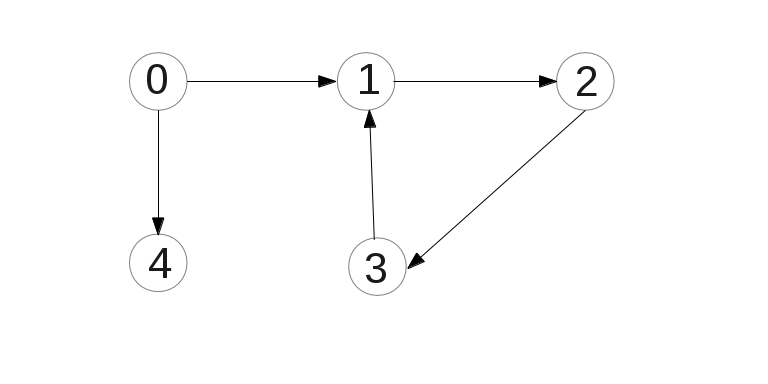
\includegraphics{immagini/test/grafoComp}
 \caption{Esempio di grafo}
 \label{fig:grafoComp}
\end{figure}

Quasi tutti i test seguono uno stesso schema; viene eseguito \textit{Trustrank} (e \textit{Anti-trust rank}) sul grafo completo, e lo indicheremo con \(t\) (\textit{Anti-trust rank} sarà indicato con \(a\)), successivamente viene eseguita la BFS (ovvero la visita in ampiezza) con nodo sorgente \(s\) e quindi si ricava la coda \(q\) dei nodi visitati a partire da \(s\); dopo di che si calcola \textit{Trustrank} (e \textit{Anti-trust rank}) sul grafo ricavati lungo la visita in ampiezza formato, quindi, da un sottoinsieme di nodi \(q\), il risultato lo indicheremo con \(\hat{t}_i\) (\textit{Anti-trust rank} sarà indicato con \(\hat{a}_i\)) dove \(i\) è il numero di nodi presi in considerazione dalla coda \(q\). Questo processo viene iterato incrementando sempre di più l'intervallo \(i\) finché non si arriva alla fine della coda \(q\) dei nodi visitati partendo dal nodo \(s\). Dopo aver calcolato \(t\) e \(\hat{t}_i\) sono due vettori si possono valutare tramite la Tau di Kendall e indicheremo con \(\tau(t,\hat{
t}_i)\) la Tau di Kendall per \(t\) e \(\hat{t}_i\)  (e quindi \(\tau(a,\hat{a}_i)\) sarà la Tau di Kendall per \(a\) e \(\hat{a}_i\)). Ad esempio in figura \ref{fig:grafoComp} è rappresentato il grafo completo su cui verra calolato \(t\) e \(a\) mentre in figura \ref{fig:grafo3} è rappresentato il grafo ricavato dalla BFS eseguita sul grafo precedente partendo dal nodo 1; se si considerano tutti i nodi lungo la visita il vettore di \textit{trustrank} sarà \(\hat{t}_3\) mentre quello di \textit{anti-trust rank} sara \(\hat{a}_3\)..

 \begin{figure}
\centering
 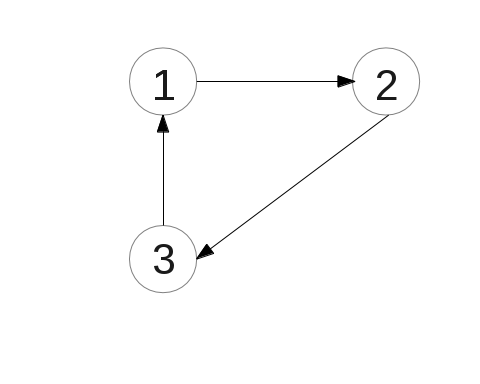
\includegraphics{immagini/test/grafo3}
 \caption{Esempio di grafo ricavato tramite una BFS a partire dal nodo 1 del grafo in figura \ref{fig:grafoComp}.}
 \label{fig:grafo3}
\end{figure}
A ogni indice del  vettore di \textit{Trustrank} \(t\) e del vettore di \textit{Anti-trust rank} \(a\) corrisponderà un nodo è il valore del vettore per un dato indice indica il valore di \textit{Trustrank} e \textit{Anti-trust rank} del nodo del grafo. In figura \ref{fig:tVettore} è illustrato un esempio del vettore di \textit{trustrank} calcolato sull'intero grafo e in figura \ref{fig:aVettore} è illustrato un esempio del vettore di \textit{anti-trust rank} calcolato sull'intero grafo. 
Nell'esempio in figura \ref{fig:tVettore} si nota che il vettore \(t\) di \textit{trustrank} ha lunghezza 5, quindi il grafo sarà composto da 5 nodi dove ad ogni nodo è associato il valore di \textit{trustrank}. Le stesse considerazioni valgono per l'esempio in figura \ref{fig:aVettore} dove il vettore di \textit{anti-trust rank} è ha lunghezza 5 e quindi l'algoritmo opererà su un grafo composto da 5 nodi.

\begin{figure}
\centering
 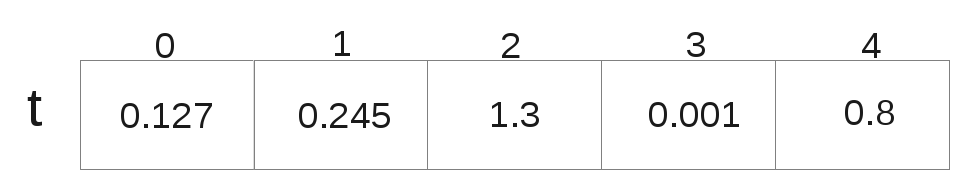
\includegraphics{immagini/test/trustVettore}
 \caption{Esempio del vettore di trustrank calcolato sull'intero grafo}
 \label{fig:tVettore}
\end{figure}
\begin{figure}
\centering
 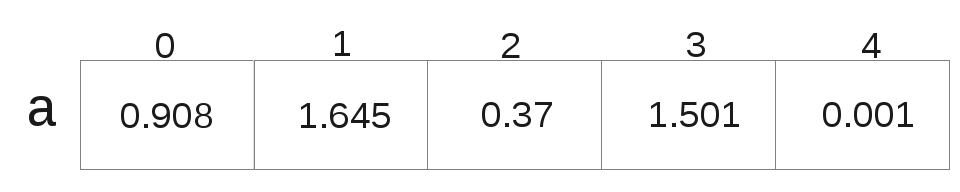
\includegraphics{immagini/test/immagineAntiTrust}
 \caption{Esempio del vettore di anti-trust rank calcolato sull'intero grafo}
 \label{fig:aVettore}
\end{figure}

A differenza dei vettori \(t\) e \(a\) (\textit{trustrank} eseguito sull'intero grafo e \textit{anti-trust rank} sull'intero grafo) , dove ad ogni indice (cioè ad ogni nodo) è associato un valore di \textit{trustrank} e \textit{anti-trust rank} , i vettori \(\hat{t}_i\) e \(\hat{a}_i\) non avranno per ogni indice un valore associato. Più precisamente, sapendo che \(\hat{t}_i\) e \(\hat{a}_i\) sono calcolati durante l'esecuzione di una BFS allora a ogni passo ci saranno ancora dei nodi da visitare per cui non è possibile calcolare i valori di \textit{trustrank} e \textit{anti-trust rank}. Quindi a ogni passo (quindi ogni qual volto vengono visitati un certo numero di nodi) sempre più nodi avranno associato un valore di \textit{trustrank} e \textit{anti-trust rank}, quindi \(\hat{t}_{i+1}\) avrà molti più nodi per cui è stato calcolato \textit{trustrank} rispetto a \(\hat{t}_i\) (questo vale anche per \textit{anti-trust rank}). Ma non è detto che dopo aver finalizzato la BFS partendo da un nodo \(s\) si sia 
visitato tutto il grafo (ovvero che \(s\) può raggiungere tutti i nodi del grafo) perciò in questo caso \(\hat{t}_i\) e \(\hat{a}_i\) avranno un numero minore di nodi per cui è calcolato \textit{trustrank} e \textit{anti-trust rank} rispetto a \(t\) e \(a\). Per gestire questa situazione i casi in cui gli indici non abbiano associato un valore ovvero quando la visita non ha ancora raggiunto tali nodi sono stati implementati due metodi.\\ 
Il primo metodo che chiameremo \textit{Modo\_A} assegna ad ogni indice dei vettori \(\hat{t}_i\) e \(\hat{a}_i\) non ancora visitato il valore 0.0. Ad esempio prendendo in considerazione il grafo in figura \ref{fig:grafoComp} e ipotizzando di eseguire una BFS a partire dal nodo 1 e di aver visitato i nodi 2 e 3 quindi se calcoliamo \textit{trustrank} e \textit{anti-trust rank} sul sottografo ricavato dai nodi visitati, i nodi 0 e 4 avranno associato i valori 0.0 (usando il metodo \textit{Modo\_A}), tale esempio è illustrato in figura \ref{fig:tBFSmodoA} e in figura \ref{fig:aBFSmodoA}.
\begin{figure}
\centering
 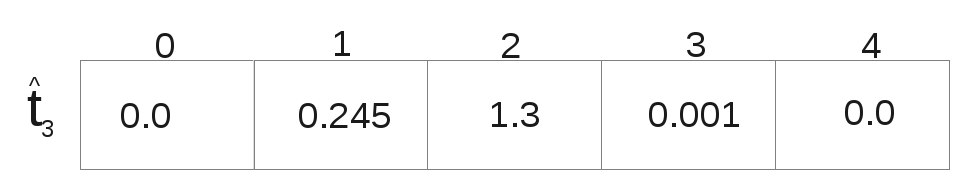
\includegraphics{immagini/test/tBFSmodoA}
 \caption{\textit{Modo\_A}. Esempio del vettore di trustrank calcolato su una porzione di grafo.}
 \label{fig:tBFSmodoA}
\end{figure}
\begin{figure}
\centering
 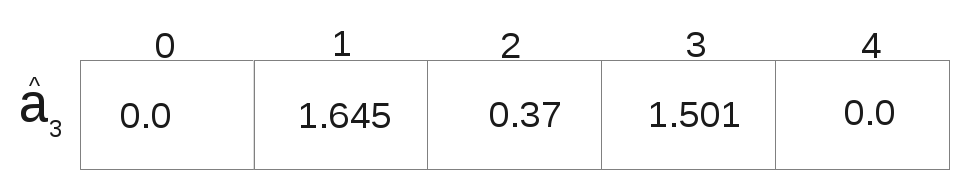
\includegraphics{immagini/test/aBFSmodoA}
 \caption{\textit{Modo\_A}. Esempio del vettore di anti-trust rank calcolato su una porzione di grafo.}
 \label{fig:aBFSmodoA}
\end{figure}
\\
Il secondo metodo che chiameremo \textit{Modo\_B} invece di assegnare il valore 0.0 ai nodi per cui non è possibile calcolare \textit{trustrank} e \textit{anti-trust rank} elimina tali indici dal vettore.  Ad esempio in figura \ref{fig:tBFSmodoB} viene illustrato il caso in cui eseguendo la BFS dal nodo 1, i nodi 0 e 4 rimangano senza aver assegnato un valore di \textit{trustrank}. Quindi gli indici 0 e 4 del vettore \(t\) non sono inclusi nel vettore \(\hat{t}_3\) questo implica che ci deve essere una corrispondenza tra gli indice del vettore \(t\) e quelli del vettore \(\hat{t}_3\) (in figura \ref{fig:tBFSmodoB} l'indice 0 del vettore \(\hat{t}_3\) corrisponde all'indice 1 del vettore \(t\), l'indice 1 al indice 2 ed infine l'indice 2 all'indice 3).  Si inoltre nota che il vettore \(\hat{t}_3\) ha lunghezza inferiore al vettore \(t\). 
\begin{figure}
\centering
 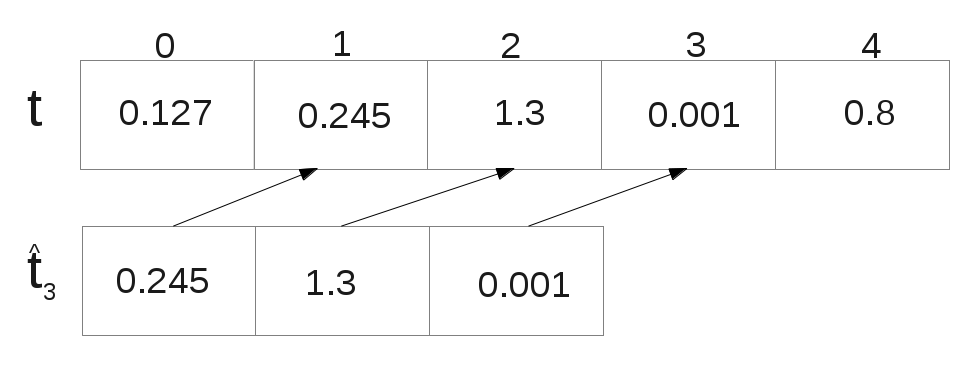
\includegraphics{immagini/test/tBFSmodoB}
 \caption{\textit{Modo\_B}. Esempio del vettore di trustrank calcolato su una porzione di grafo.}
 \label{fig:tBFSmodoB}
\end{figure}

Quindi la valutazione tra il vettore di \(t\), di \textit{trustrank}, calcolato sul grafo completo e il vettore \(\hat{t}_i\), di \textit{trustrank}, calcolato su una parte del grafo può avveniere usando ho il \textit{Modo\_A} o il \textit{Modo\_B}. Nel caso della valutazione nel \textit{Modo\_B} il vettore \(t\) dovra essere ristretto alla lunghezza del vettore \(\hat{t}_i\) e quindi dovranno essere eliminati gli indici del vettore \(t\) che non sono inclusi nel vettore \(\hat{t}_i\).
%parlare del fatto che al vettore d nel modoA bisogna togliere gli indici che non servono

I test saranno, quindi, cosi strutturari:
\begin{itemize}
 \item Test numero 1. Si confronta \textit{trustrank} sul grafo completo con \textit{trustrank} calcolato su una porzione di grafo. Lo stesso si fa per \textit{anti-trust ran}.
 \item Test numero 2. Si confrontano i solo nodi etichettati spam del vettore di  \textit{trustrank} sul grafo completo con  i soli nodi etichettati spam del vettore di \textit{trustrank} calcolato su una porzione di grafo. Nel caso di \textit{anti-trust rank} si  confrontano i nodi etichettati come non spam.
 \item Test numero 3. Si calcola \textit{trustrank} sul grafo completo ottenuto eseguendo la visita partendo da un nodo \(s\) e si confronta con \textit{trustrank} eseguito a ogni passo delle visita ma si imposta un seedset diverso formato dagli ultimi \(n\) nodi della vista. Viene applicato lo stesso metodo per \textit{anti-trust rank}.
 \item Test numero 4. Si esegue la BFS a partire dal nodo \(s\) e per ogni passo si calola la media dei valori di \textit{trustrank} dei soli nodi che sappiamo essere non spam e la media dei valori di \textit{Trustrank} dei soli nodi spam. Quindi si calcola la differenza tra le due medie. Lo stesso metodo verrà applicato per l'analisi dell'algoritmo di \textit{anti-trust rank}.
 \end{itemize}

 Dal momento che i test 1, 2 e 3 utilizzano la Tau di Kendall per calcolare la distanza tra i vettori \(t\) e \(\hat{t}_i\) allora ognuno dei test verra eseguito secondo il \textit{Modo\_A} e il \textit{Modo\_B}.
 
 \section{Test 1}
 Questo test calcola la distanza tra il vettore \(t\) di \textit{trustrank} ricavato sull'intero grafo e il vettore \(\hat{t}_i\) di \textit{trustrank} calcolato sul grafo ricavato dai nodi visitati lungo una visita in ampiezza con nodo sorgente \(s\). Inoltre viene eseguto lo stesso procedimento per quanto riguarda \textit{anti-trust rank} ovvero si calcolano le distanze tra il vettore di \(a\) di \textit{anti-trust rank} ottenuto dal grafo completo e il vettore \(\hat{a}_i\)  caloato sul grafo ricavato dai nodi visitati lungo  un visita in ampiezza con nodo sorgente \(s\). Dal dataset sono impostati come nodo sorgente della BFS due nodi: il nodo 62 etichettato come non spam e il nodo 112 etichettato come spam. Inoltre per il calcolo di \textit{trustrank} sull'intero grafo viene utilizzato come seedset l'insieme di pagine del dataset WEBSPAM-UK2007 etichettate come non spam mentre per il calcolo di \textit{trustrank} sul grafo ottenuto dai nodi visitati durante la BFS il seedset sarà formato dalle pagine 
visitate che sono etichettate come non spam nel dataset WEBSPAM-UK2007. Per il calolo di \textit{anti-trust rank} sull'intero grafo, invece, il seedset sarà composto dalle pagine etichettate come spam nel dataset WEBSPAM-UK2007 mentre il seedset di \textit{anti-trust rank} calcolato sul grafo ottenuto dai nodi visitati dalla BFS sarà formato dai soli nodi visitati che sono etichettati come spam.
 \subsection{Modo\_A}

 In figura \ref{fig:test1trustModoA62} è illustrato il grafico risultante della Tau di Kendall , calcolata usando il \textit{Modo\_A}, tra \(t\) e \(\hat{t}_i\) dove la visita in ampiezza ha come nodo sorgente il nodo 62, allo stesso modo in figura \ref{fig:test1trustModoA112} è illustrato il grafico risultante tra la Tau di Kendall, calcolata usando il \textit{Modo\_A}, di \(t\) e \(\hat{t}_i\) calcolato sul grafo ottenuto lungo una visita in ampiezza con nodo sorgente 112. Sull'asse delle ascisse è rappresentato il numero di nodi che sono stati visitati attraverso la BFS e quindi il numero di nodi del grafo su cui è stato calcolato \(\hat{t}_i\) dove \(i\) è appunto il numero di nodi presi in considerazione, mentre sull'asse delle ordinate è rappresentato il valore della Tau di Kendall tra il vettore \(t\) e \(\hat{t}_i\).
 %parlare dell'intervallo con cui vengono incrementati i nodi?
 
 Quello che si nota è che quando la visita è nella fase iniziale e quindi il grafo risultante è costituito da pochi nodi rispetto al grafo completo, il valore della Tau di Kendall è prossimo allo 0 ma questo valore cresce in modo proporzionale al numero di nodi visitati lungo la BFS fino ad arrivare a circa il valore massimo ovvero 1. Inoltre l'andamento del grafico mostra che quando si arriva a meta dei nodi visitati la Tau di Kendall è uguale a circa 0.5 e questo implica che gia dopo aver visitato la metà dei nodi del grafo si può utilizzare \textit{trustrank} in modo online ed avere un il vettore risultatnte molto simile al vettore di \textit{trustrank} calcolato sul grafo completo ovvero la distanza tra i due vettori è breve. Tale distanza sarà sempre più breve quanto più la visita in ampiezza, e quindi il crawler, visiterà le pagine.

  \begin{figure}
\centering
 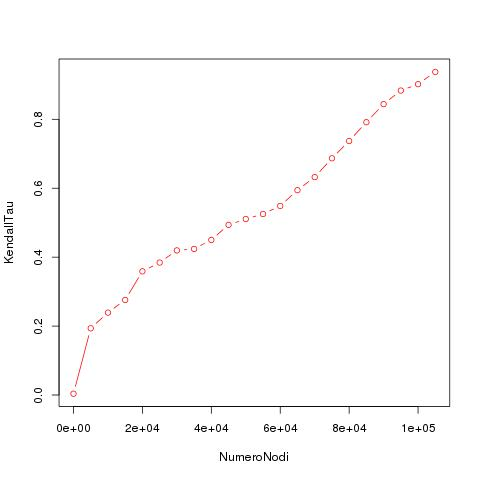
\includegraphics[height=9cm]{immagini/test1/trustranktestMode0_62}
 \caption{Test numero 1 (trustrank, 62). Calcolo della distanza dei vettori, usando il Modo\_A, tra trustrank calcolato sull'intero grafo e trustrank calcolato sul grafo ricavato dai nodi visitati lungo una BFS partendo dal nodo 62.}
 \label{fig:test1trustModoA62}
\centering
 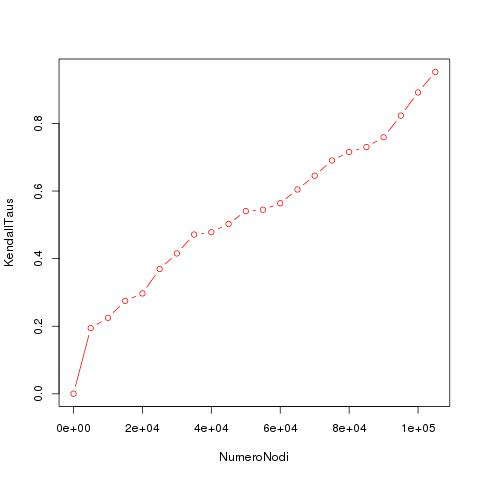
\includegraphics[height=9cm]{immagini/test1/trustranktestMode0_112}
 \caption{Test numero 1 (trustrank, 112). Calcolo della distanza dei vettori, usando il Modo\_A, tra trustrank calcolato sull'intero grafo e trustrank calcolato sul grafo ricavato dai nodi visitati lungo una BFS partendo dal nodo 112.}
 \label{fig:test1trustModoA112}
\end{figure}
 
Quanto descritto per la fase di testing di \textit{trustrank} vale per \textit{anti-trust rank}. In figura \ref{fig:test1antitrustModoA62} è illustrato il grafico risultante della Tau di Kendall , cacolata usando il \textit{Modo\_A}, tra il vettore di \textit{anti-trust rank} calcolato sull'intero grafo e il vettore di \textit{anti-trust rank} calcolato sul grafo ottento dai nodi visitati attraverso la BFS con nodo sorgente 62, mentre in figura \ref{fig:test1antitrustModoA112} il nodo sorgente della BFS è 112. Anche questi due grafici mostrano che quanto più la visita BFS cresce tanto più i vettori \(a\) e \(\hat{a}_i\) sono simili. Quindi la distanza tra il vettore \(a\) e \(\hat{a}_i\) è minore tanto più la visita entra in profondità del grafo.

Quindi il comportamento di \textit{trustrank} e \textit{anti-trust rank} in modalità online è fortemente dipendende dalla proporzione di grafo che si sta esaminando. 
  
 \begin{figure}
\centering
 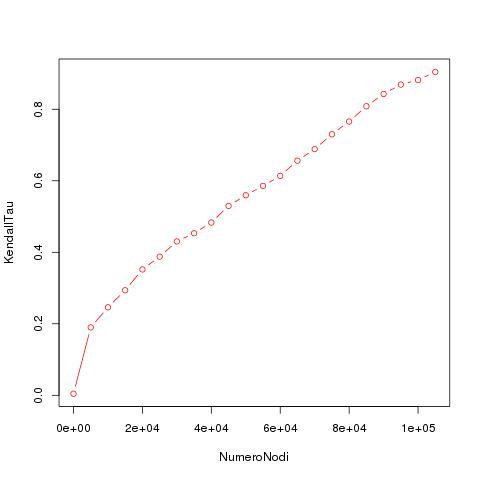
\includegraphics[height=9cm]{immagini/test1/antiTrustrankTestMode0_62}
 \caption{Test numero 1 (anti-trust rank, 62). Calcolo della distanza dei vettori, usando il Modo\_A, tra anit-trust rank calcolato sull'intero grafo e anti-trust rank calcolato sul grafo ricavato dai nodi visitati lungo una BFS parteneo dal nodo 62.}
 \label{fig:test1antitrustModoA62}
\centering
 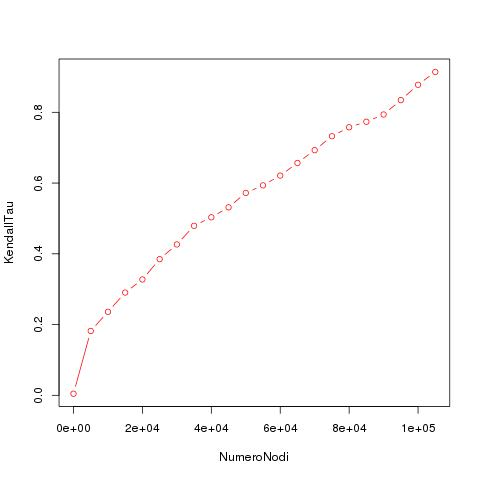
\includegraphics[height=9cm]{immagini/test1/antiTrustrankTestMode0_112}
 \caption{Test numero 1 (anti-trust rank, 112). Calcolo della distanza dei vettori, usando il Modo\_A, tra anit-trust rank calcolato sull'intero grafo e anti-trust rank calcolato sul grafo ricavato dai nodi visitati lungo una BFS parteneo dal nodo 112.}
 \label{fig:test1antitrustModoA112}
\end{figure}

\subsection{Modo\_B}
I risultati ottenuti fino adesso non sono completamente veritieri in quanto nel \textit{Modo\_A} alcuni indici del  vettore \(\hat{t}_i\) e alcuni indici del vettore \(\hat{a}_i\) potrebbero aver assegnato il valore 0.0 nel caso in cui questi non siano stati visitati dalla BFS. Quindi si evince che la Tau di Kendall sarà influenzata da tale meccanismo ed ecco perché è si è scelto di gestire i valori dei due vettori \(\hat{t}_i\) e \(\hat{a}_i\) attraverso il \textit{Modo\_B}.

In figura \ref{fig:test1trustModoB62} e in figura \ref{fig:test1trustModoB112} sono rappresentati rispettivamente i grafici delle Tau di Kendall gestite tramite il \textit{Modo\_B}, per il cacolo delle distanze tra il vettore \(t\) calcolato sull'intero grafo e il vettore \(\hat{t}_i\) calcolato sul grafo ottenuto dai nodi visitati lungo una visita in ampiezza con nodo sorgente nel primo caso 62 e nel secondo 112.  Anche in questo caso sull'asse delle ascisse è rappresentato il numero di nodi che sono stati visitati attraverso la BFS e quindi il numero di nodi del grafo su cui viene calcolato \(\hat{a}_i\) dove \(i\) è appunto il numero di nodi presi in considerazione, mentre sull'asse delle ordinate è rappresentato il valore della Tau di Kendall tra il vettore \(t\) e \(\hat{t}_i\).
La Tau di Kendall si comporta differentemente dai risultati ottenuti nel \textit{Modo\_A} (in particolare figura \ref{fig:test1trustModoA62} e \ref{fig:test1trustModoA112}): il valore di Tau di Kendall uguale ad 1 si ha quando la BFS ha visitato il solo nodo di partenza, dal momento che il vettore \(t\) ha un solo indice e il vettore \(\hat{t}_1\) ha un solo indice il confronto con la Tau di Kendall ritorna un valore uguale ad 1. Dopo aver visitato il primo nodo l'andamento del grafico segue quello visto nel \textit{Modo\_A} dove all'aumentare dei nodi visitati della BFS il i vettore \(t\) e \(\hat{t}_i\) sono sempre meno distanti. Si nota inoltre che usando il \textit{Modo\_B} i valori dell Tau di Kendall (escludendo il caso della visit di un unico nodo) in entrambi i grafici \ref{fig:test1trustModoB62} e \ref{fig:test1trustModoB112} incominciano intorno a 0.7 per pochi nodi visitati e si arriva ad avere valore uguale a circa 1 alla fine della visita differentemente dal \textit{Modo\_A} dove il valore della 
Tau di Kendall cresce da 0 a circa 1. Il motovo di tale comportamento risiede nel modo con cui vengono trattati i vettori nei due modi: \textit{Modo\_A} e \textit{Modo\_B}. Più precisamente mentre nel \textit{Modo\_A} agli indici, del vettore \(\hat{t}_i\) e \(\hat{a}_i\), che non sono stati visitati dalla BFS è assegnato il valore 0.0 e la lunghezza del vettore \(\hat{t}_i\) e del vettore \(\hat{a}_i\) è uguale al numero dei nodi dell'intero grafo nel \textit{Modo\_B} i vettori \(\hat{t}_i\) e \(\hat{a}_i\) sono ridimensionati ai soli nodi visitati dalla BFS questo implica che anche i vettori \(t\) e \(a\), ottenuti dall'elaborazione dell'intero grafo, vengano ridimensionati alla stessa lunghezza considerando i soli nodi visitati dalla BFS. Quindi mentre nel primo caso i due vettori per cui viene calcolata la Tau di Kendall sono distanti tra loro all'inizio della BFS in quanto avranno molti valori dicordanti in quanto ai vettori \(\hat{t}_i\) e \(\hat{a}_i\) vengono asseganti dei valori non veritieri (il 
valore 0.0) ai nodi non ancora visitati nel secondo metodo il confronto è fatto solo tra i valori dei nodi del grafo temporaneo ottenuto dalla BFS e il valori dei nodi del grafo completo che sono inclusi nel grafo temporano. 
 \begin{figure}
\centering
 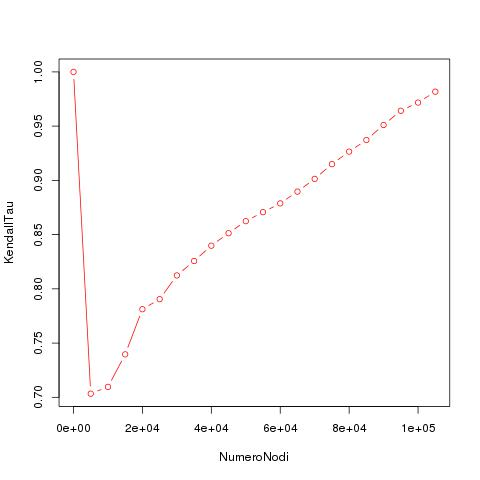
\includegraphics[height=9cm]{immagini/test1/trustranktestMode1_62}
 \caption{Test numero 1 (trustrank, 62). Calcolo della distanza dei vettori, usando il Modo\_B, tra trustrank calcolato sull'intero grafo e trustrank calcolato sul grafo ricavato dai nodi visitati lungo una BFS partendo dal nodo 62.}
 \label{fig:test1trustModoB62}
\centering
 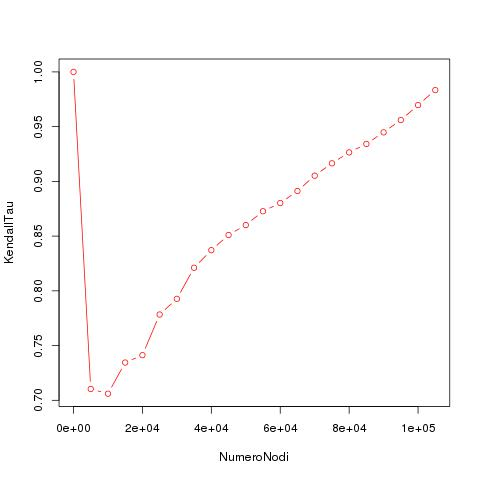
\includegraphics[height=9cm]{immagini/test1/trustranktestMode1_112}
 \caption{Test numero 1 (trustrank, 112). Calcolo della distanza dei vettori, usando il Modo\_B, tra trustrank calcolato sull'intero grafo e trustrank calcolato sul grafo ricavato dai nodi visitati lungo una BFS partendo dal nodo 112.}
 \label{fig:test1trustModoB112}
\end{figure}

Eseguendo lo stesso test per valutare la distanza tra il vettore \(a\) di \textit{anti-trust rank} calcolato sull'intero grafo e il vettore \(\hat{a}_i\) calcolato sul grafo ottenuto dai nodi visitati durante una visita in ampiezza si nota che i risultati sono presocchè uguali ai precedenti due test. In particolare in figura \ref{fig:test1antitrustModoB62} è rappresentato il grafico della Tau di Kendall che mette a confronto il vettore \(a\) con il vettore \(\hat{a}_i\) dove la BFS ha come nodo sorgente 62 mentre in figura \ref{fig:test1antitrustModoB112} è rappresentato il grafico della Tau di Kendall che mette a confronto il vettore \(a\) con il vettore \(\hat{a}_i\) dove la BFS ha nodo sorgente 112; sull'asse delle ascisse è rappresentao il numero di nodi che sono visitati durante la BFS mentre sulle ordinate il corrispondente valore di Tau di Kendall tra il vettore di \(a\) calcolato sull'intero grafo e il vettore \(\hat{a}_i\) calcolato sul grafo ricavato dai nodi visitati attraverso una BFS a diversi 
passi, quindi \(i\) sarà uguale al numero dei nodi visitati ad un certo istante. Rispetto al test di \textit{trustrank} usando \textit{anti-trust rank} si nota che i grafici (senza considerare il primo valore per lo stesso motivo dei due test precedenti) hanno un andamento quasi logaritmico dove si ha come valore iniziale di Tau di Kendall 0.75 e come utlimi valori (stazionari) 0.95. Infatti un fattore evidente è che la Tau di Kendall tende a non superare il 0.95 per gli ultimi nodi incontrati nella BFS.

 \begin{figure}
\centering
 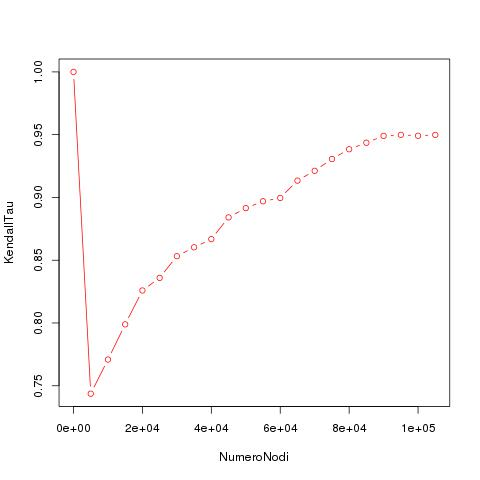
\includegraphics[height=9cm]{immagini/test1/antiTrustrankTestMode1_62}
 \caption{Test numero 1 (anti-trust rank, 62). Calcolo della distanza dei vettori, usando il Modo\_B, tra anit-trust rank calcolato sull'intero grafo e anti-trust rank calcolato sul grafo ricavato dai nodi visitati lungo una BFS parteneo dal nodo 62.}
 \label{fig:test1antitrustModoB62}
\centering
 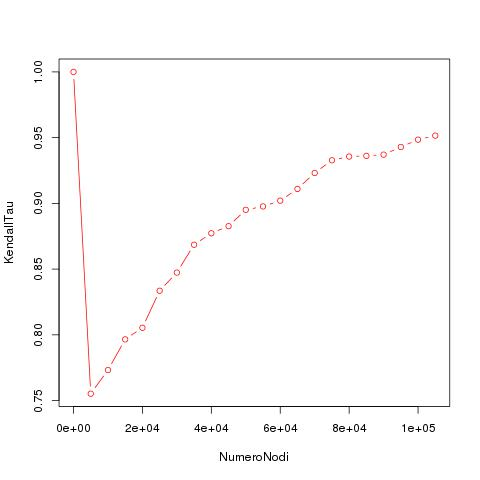
\includegraphics[height=9cm]{immagini/test1/antiTrustrankTestMode1_112}
 \caption{Test numero 1 (anti-trust rank, 112). Calcolo della distanza dei vettori, usando il Modo\_B, tra anit-trust rank calcolato sull'intero grafo e anti-trust rank calcolato sul grafo ricavato dai nodi visitati lungo una BFS parteneo dal nodo 112.}
 \label{fig:test1antitrustModoB112}
\end{figure}

\newpage
In figura \ref{fig:test1coplot62} sono riportati in un unico grafico i grafici rappresentati in figura \ref{fig:test1trustModoB62} e del  grafico \ref{fig:test1antitrustModoB62}; in rosso è rappresentato il grafico \ref{fig:test1trustModoB62} relativo alla Tau di Kendall tra \textit{trustrank} calcolato sull'intero grafo e \textit{trustrank} calcolato sul grafo ottenuto dai nodi visitati a diversi passi di una BFS con nodo sorgente 62 mentre in verde è rappresentato il grafico  \ref{fig:test1antitrustModoB62} relativo alla Tau di Kendall tra \textit{anti-trust rank} calcolato sull'intero grafo e \textit{anti-trust rank} calcolato sul grafo ottenuto dai nodi visitati a diversi passi di una BFS con nodo sorgente 62. Quello che evince è che la Tau di Kendall applicata al vettore \(a\) e \(\hat{a}_i\) cresce più velocemente rispetto a quella applicata a \(t\) e \(\hat{t}_i\) quindi tra \textit{trustrank} e \textit{anti-trust rank} il miglior metodo per essere utilizzato in modalità online è il secondo perché \
textit{anti-trust rank} tende ad approssimare meglio il comportamento offline. Infatti il grafico in figura \ref{fig:test1coplot62} indica che \textit{anti-trust rank} eseguito durante la fase di crawling ritorna un vettore dove i valori tendono ad avvicinarsi rapidamente ai valore del vettore se \textit{anti-trust rank} fosse eseguito in modalità offline. Le stesse valutazioni valgono tra il confronto dei due grafici in figura \ref{fig:test1trustModoB112} e \ref{fig:test1antitrustModoB112} illustrato in figura \ref{fig:test1coplot112} dove in rosso è rappresentata la Tau di Kendall  tra \textit{trustrank} calcolato sull'intero grafo e \textit{trustrank} calcolato sul grafo ottenuto dai nodi visitati a diversi passi di una BFS con nodo sorgente 112 mentre in verde è rappresentato il la Tau di Kendall tra \textit{anti-trust rank} calcolato sull'intero grafo e \textit{anti-trust rank} calcolato sul grafo ottenuto dai nodi visitati a diversi passi di una BFS con nodo sorgente 112.

 \begin{figure}
\centering
 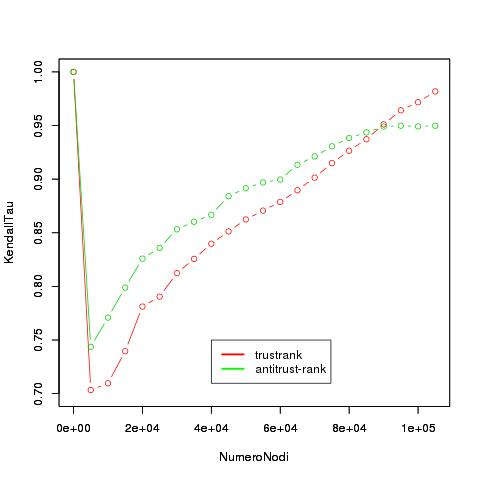
\includegraphics[height=9cm]{immagini/test1/coplotTrustAnti_62}
 \caption{Plotting del grafico \ref{fig:test1trustModoB62} e del  grafico \ref{fig:test1antitrustModoB62}}
 \label{fig:test1coplot62}
\centering
 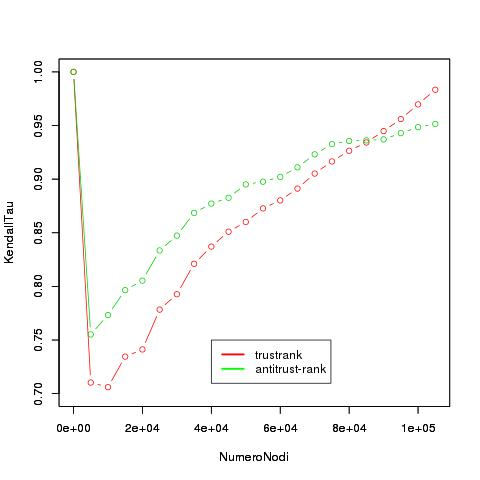
\includegraphics[height=9cm]{immagini/test1/coplotTrustAnti_112}
 \caption{Plotting del grafico \ref{fig:test1trustModoB112} e del  grafico \ref{fig:test1antitrustModoB112}}
 \label{fig:test1coplot112}
\end{figure}

\section{Test 2}
Il test consiste nel valutare la distanza tra due vettori, il vettore \(t\) di \textit{trustrank} calcolato sull'intero grafo e il vettore \(\hat{t}_i\) calcolato sul grafo ottentuto dai nodi visitati durante un visita in ampiezza; quindi la distanza viene calcolata ogni qual volta il numero di indici, del vettore \(\hat{t}_i\), a cui è possibile associare un valore aumenta  di un certo intervallo ovvero  quando la BFS visita un intervallo di nodi stabilito adentrandosi sempre di più nel grafo. Il test cosi descritto è simile al \textit{Test numero 1} ma differentemente del precedente in questo test nel determinare la distanza tra i due vettori si esaminano i soli indici che fanno riferimento ai nodi etichettati come spam. Ugualmente il test viene effettuato per valutare \textit{anti-trust rank} ma in questo caso vengono confrontati i soli nodi indici dei due vettore \(a\) e \(hat{a}_i\) che fanno riferimento a nodi etichettati come non spam.

Anche per questo test nella valutazione di \textit{trustrank} è stato usato come seedset l'insieme dei nodi etichettati non spam del dataset WEBSPAM-UK2007 mentre per \textit{anti-trustrank} è stato usto come seedset l'insieme dei nodi spam del dataset WEBSPAM-UK2007.

\subsection{Modo\_A}

\begin{figure}
\centering
 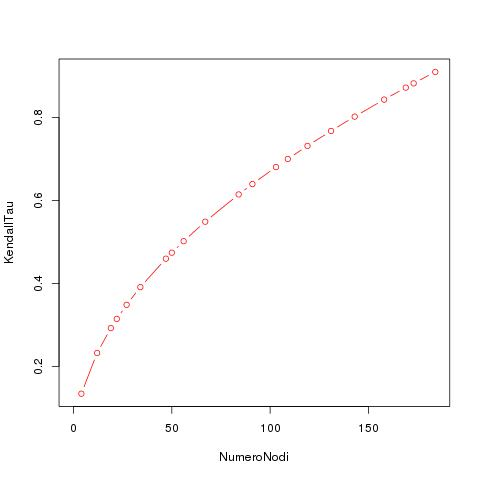
\includegraphics[height=9cm]{immagini/test2/trustrankBadNodesTestMode0_62}
 \caption{Test numero 2 (trustrank, 62). Calcolo della distanza dei vettori, usando il Modo\_A, tra trustrank calcolato sull'intero grafo e trustrank calcolato sul grafo ricavato dai nodi visitati lungo una BFS partendo dal nodo 62 prendendo in considerazione i soli nodi spam. }
 \label{fig:test2trustModoA62}
\centering
 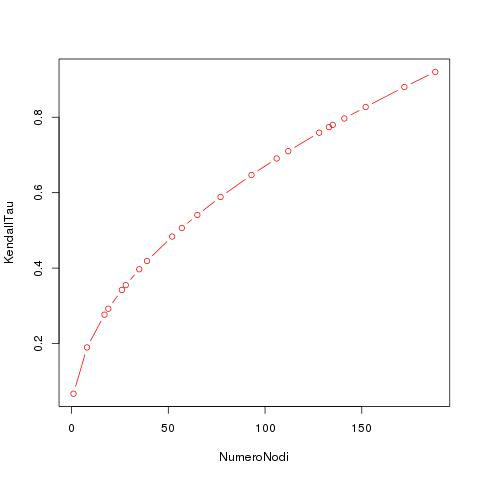
\includegraphics[height=9cm]{immagini/test2/trustrankBadNodesTestMode0_112}
 \caption{Test numero 2 (trustrank, 112). Calcolo della distanza dei vettori, usando il Modo\_A, tra trustrank calcolato sull'intero grafo e trustrank calcolato sul grafo ricavato dai nodi visitati lungo una BFS partendo dal nodo 112 prendendo in considerazione i soli nodi spam.}
 \label{fig:test2trustModoA112}
\end{figure}

Il test calcola la distanza tra i soli indici del vettore \(t\) di \textit{trustrank}, ottenuto sull'analisi dell'intero grafo, che fanno riferimento a nodi spam e i gli indici del vettore \(\hat{t}_i\) di \textit{trustrank}, ottenuto dall'analisi del grafo ricavato ogni intervallo di nodi visitato tramite una visita in ampiezza, che fanno riferimento a nodi spam.

I risultati del test effettuato su \textit{trustrank}, usando il \textit{Modo\_A}, sono illustrati in figura \ref{fig:test2trustModoA62} e in figura \ref{fig:test2trustModoA112}; nel primo grafico il nodo sorgente della visita in ampiezza, che viene utilizzata per costruire il grafo temporaneo ogni intervallo di nodi visitati e su cui viene calcolato \(\hat{t}_i\) ad ogni intervallo, è il nodo 62 mentre nel secongo grafico il nodo è 112.  Sull'asse delle ascisse sono rappresentati il numero di nodi che sono spam tra quelli che vengono visitati tramite la visita in ampiezza mentre sull'asse delle ordinate è rappresentato il valore della Tau di Kendall tra i nodi spam del vettore \(t\) e i nodi spam del vettore \(\hat{t}_i\), calcolata a ogni intervallo di nodi visitati tramite la visita in ampiezza.\\
Entrambi i grafici evidenziano che all'aumentare di nodi visitati attraverso la visita in ampiezza e quindi all'aumentare del grafo temporaneo su cui viene calcolato \(\hat{t}_i\), il vettore \(\hat{t}_i\) ha i valore dei nodi spam che sono molto più vicini ai vaolori de nodi spam del vettore \(\hat{t}_i\); infatti si nota che verso la fine della visita la Tau di Kendall dei valori dei nodi del vettore \(t\) con i valori dei nodi spam del vettore \(\hat{t}_i\) è circa 1. 

Quanto descritto per l'analisi di \textit{trustrank} vale per \textit{anti-trust rank}. In figura in figura \ref{fig:test2antitrustModoA62} e in figura \ref{fig:test2antitrustModoA112} sono illustrati i grafici relativi alla Tau di Kendall tra i gli indici dei nodi non spam del vettore \(a\) di \textit{anti-trust rank}, calcolato sull'intero grafo, e gli indici  del vettore \(\hat{a}_i\) di \textit{trustrank}, ottenuto dall'analisi del grafo ricavato ogni intervallo di nodi visitato tramite una visita in ampiezza, che fanno riferimento a spam; Nel primo grafico il nodo sorgente della visita in ampiezza è 62 mentre nel secondo è 112. Sull'asse delle ascisse sono rappresentati il numero di nodi non spam tra i nodi visitati tramite la visita in ampiezza mentre sull'asse mentre sull'asse delle ordinate è rappresentato il valore della Tau di Kendall tra nodi non spam del vettore \(a\) e i nodi non spam del vettore \(\hat{a}_i\).\\
La  Tau di Kendall tra i nodi non spam del vettore \(a\) e del vettore \(\hat{a}_i\) cresce sempre di più con l'aumentare dei nodi visitati attrverso la visita in ampiezza fino ad arrviare a circa uno quando quasi tutto il grafo è stato visitato e quindi il valore di \(\hat{a}_i\) riprodurrà quasi fendelemnte i valori del vettore \(a\). Questo fattore è duvuto al fatto che il grafo temporaneo ricavato dai nodi visitati tramite la visita in ampiezza sarà sempre più simile al grafo completo tanto più la visita entra in profondità e quindi \textit{anti-trust rank} calcolato su tale grafo riprodurrà sempre più con maggiore affidabilità i valori calcolati sull'intero grafo.


\begin{figure}
\centering
 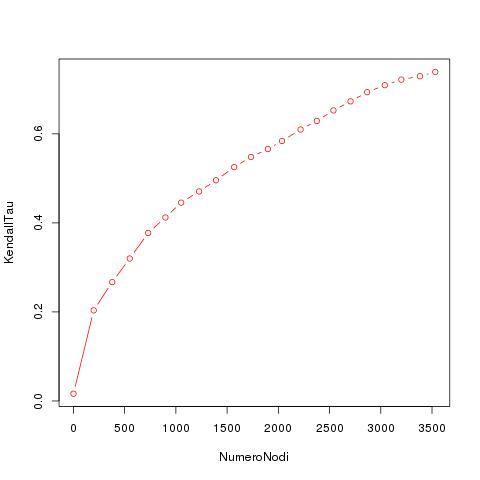
\includegraphics[height=9cm]{immagini/test2/antiTrustraktGoodNodesTestMode0_62}
 \caption{Test numero 2 (anti-trust rank, 62). Calcolo della distanza dei vettori, usando il Modo\_A, tra anti-trust rank calcolato sull'intero grafo e anti-trust rank calcolato sul grafo ricavato dai nodi visitati lungo una BFS partendo dal nodo 62 prendendo in considerazione i soli nodi non spam. }
 \label{fig:test2antitrustModoA62}
\centering
 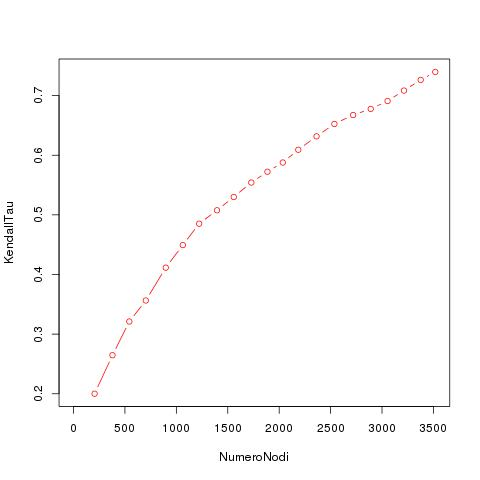
\includegraphics[height=9cm]{immagini/test2/antiTrustraktGoodNodesTestMode0_112}
 \caption{Test numero 2 (anti-trust rank, 62). Calcolo della distanza dei vettori, usando il Modo\_A, tra anti-trust rank calcolato sull'intero grafo e anti-trust rank calcolato sul grafo ricavato dai nodi visitati lungo una BFS partendo dal nodo 112 prendendo in considerazione i soli nodi non spam. }
 \label{fig:test2antitrustModoA112}
\end{figure}

\subsection{Modo\_B}
Anche nel \textit{Modo\_B} il test determina la distanza tra i soli indici del vettore \(t\) di \textit{trustrank} (o dei soli indici del vettore \(a\) nel caso di \textit{anti-trust rank}), ottenuto sull'analisi dell'intero grafo, che fanno riferimento a nodi spam e i gli indici del vettore \(\hat{t}_i\) di \textit{trustrank} (o dei soli indici del vettore \(\hat{a}_i\) nel caso di \textit{anti-trust rank}), ottenuto dall'analisi del grafo ricavato ogni intervallo di nodi visitato tramite una visita in ampiezza, che fanno riferimento a nodi spam.

In figura \ref{fig:test2trustModoB62} è rappresentato il grafico di tale esperimento dove il nodo sorgente della visita in ampiezza è 62. Dal momento che si sta eseguendo il test nel \textit{Modo\_B} ci si aspetta che (come per il test numero 1) il primo valore della Tau di Kendall (ovvero quando la BFS ha visitato solo il nodo sorgente) sia 1 ma visto che si stanno prendendo i soli nodi spam in questo caso dato che il nodo sorgente è non spam il nodo è scartato è quindi i vettore \(t\) e \(\hat{t}_i\) sono vuoti differentemente dal \textit{Modo\_A} dove ai nodi del vettore \(\hat{a}_i\) che risultavano non spam veniva assegnato il valore 0.0. Dopo di che l'andamento del grafico cresce rapidamente fino a circa 0.7 e cresce gradualemnte fino a circa 1.0. 

\begin{figure}
\centering
 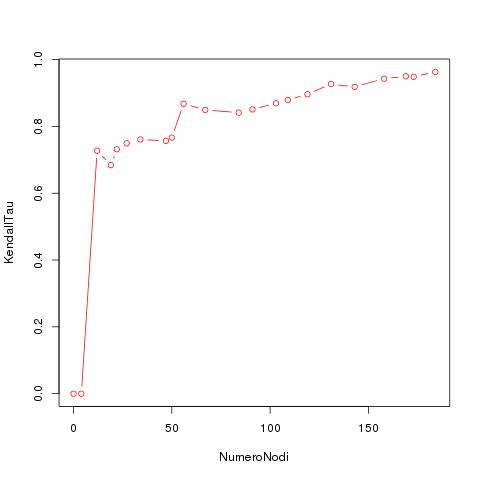
\includegraphics[height=9cm]{immagini/test2/trustrankBadNodesTestMode1_62}
 \caption{Test numero 2 (trustrank, 62). Calcolo della distanza dei vettori, usando il Modo\_B, tra trustrank calcolato sull'intero grafo e trustrank calcolato sul grafo ricavato dai nodi visitati lungo una BFS partendo dal nodo 62 prendendo in considerazione i soli nodi spam. }
 \label{fig:test2trustModoB62}
\centering
 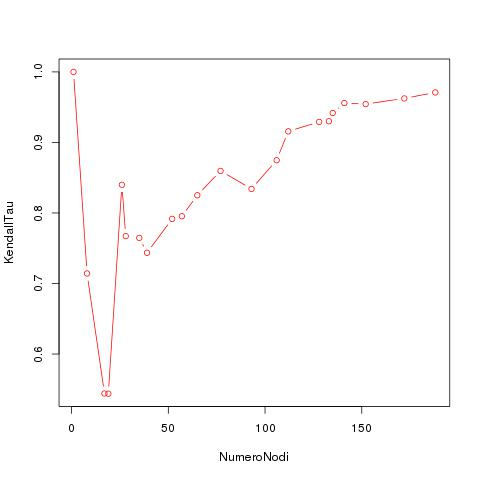
\includegraphics[height=9cm]{immagini/test2/trustrankBadNodesTestMode1_112}
 \caption{Test numero 2 (trustrank, 112). Calcolo della distanza dei vettori, usando il Modo\_B, tra trustrank calcolato sull'intero grafo e trustrank calcolato sul grafo ricavato dai nodi visitati lungo una BFS partendo dal nodo 112 prendendo in considerazione i soli nodi spam.}
 \label{fig:test2trustModoB112}
\end{figure}

\begin{figure}
\centering
 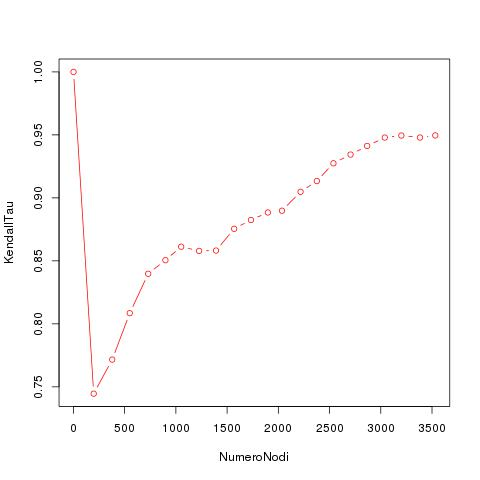
\includegraphics[height=9cm]{immagini/test2/antiTrustraktGoodNodesTestMode1_62}
 \caption{Test numero 2 (anti-trust rank, 62). Calcolo della distanza dei vettori, usando il Modo\_B, tra anti-trust rank calcolato sull'intero grafo e anti-trust rank calcolato sul grafo ricavato dai nodi visitati lungo una BFS partendo dal nodo 62 prendendo in considerazione i soli nodi non spam. }
 \label{fig:test2antitrustModoB62}
\centering
 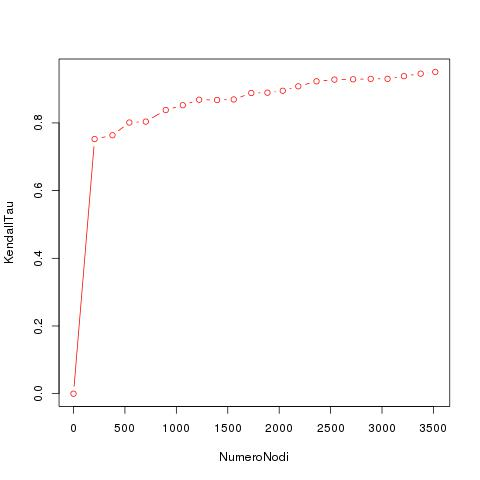
\includegraphics[height=9cm]{immagini/test2/antiTrustraktGoodNodesTestMode1_112}
 \caption{Test numero 2 (anti-trust rank, 62). Calcolo della distanza dei vettori, usando il Modo\_B, tra anti-trust rank calcolato sull'intero grafo e anti-trust rank calcolato sul grafo ricavato dai nodi visitati lungo una BFS partendo dal nodo 112 prendendo in considerazione i soli nodi non spam. }
 \label{fig:test2antitrustModoB112}
\end{figure}





